\documentclass[USenglish]{article}
\usepackage[utf8]{inputenc}
\usepackage[T1]{url}

\usepackage[a4paper]{geometry}
\usepackage{listings}

\setlength{\parskip}{1em}
\setlength{\parindent}{0em}
\usepackage{caption}
\usepackage{subcaption}
\usepackage{bookmark}

\urlstyle{sf}

\usepackage[table]{xcolor}
\usepackage{tikz,babel,textcomp,csquotes,varioref,graphicx,float}
\usepackage{rtm}
\usepackage{tikz-uml}
\usepackage{babel}
\usepackage{graphicx}
\usepackage{ifikompendiumforside}
\usepackage{hyperref}
\usepackage{array}
\usepackage[font={small,it,sf}]{caption}
\usepackage{longtable}
\usepackage{multirow}
\usepackage{wrapfig}
\usepackage{titlesec,titletoc}
\usetikzlibrary{arrows, shadows}

\newcommand{\TRUE}{\cellcolor{green}{\textbf{True}}}
\newcommand{\YES}{\cellcolor{green}{\textbf{Yes}}}
\newcommand{\FALSE}{\cellcolor{red}{\textbf{False}}}
\newcommand{\NO}{\cellcolor{red}{\textbf{No}}}
\newcommand{\NONE}{\cellcolor{gray}{\textbf{--}}}

\title{INF4121 Project Assignment 2}
\subtitle{Testing and test automation}
\author{Per Øyvind Karlsen}

\begin{document}
\ififorside

\section{Requirements}

\subsection{Manual tests}

\begin{description}
	\item \req{1}{Sign-in}{\textit{Not really an independent test..}}
		\begin{table}[ht]
			\centering
			\caption{Sign-in decission table}
			\label{signin-decission-table}
			\begin{tabular}{|c|l|c|c|c|c|}
				\hline
				\parbox[t]{3mm}{\multirow{4}{*}{\rotatebox[origin=c]{90}{Conditions}}} &
				New user 		& \TRUE	& \FALSE	& \FALSE	& \NONE		\\ \cline{2-6} &
				Valid username		& \NONE	& \FALSE	& \NONE		& \TRUE		\\ \cline{2-6} &
				Valid password		& \NONE	& \NONE		& \FALSE	& \TRUE		\\ \cline{2-6} &
				\multicolumn{5}{l|}{} \\
				\hline
				\parbox[t]{3mm}{\multirow{3}{*}{\rotatebox[origin=c]{90}{Actions}}} &
				Create user		& \YES	& \NO		& \NO		& \NO		\\ \cline{2-6} &
				Login fail (error) 	& \NO	& \YES		& \YES		& \NO		\\ \cline{2-6} &
				Login success		& \YES	& \NO		& \NO		& \YES		\\ \hline
			\end{tabular}
		\end{table}
		\newpage
		\begin{description}
			\item\req{1.1}{Register new customer}{
				In order for automatic test to pass check for missing username were excluded
				due to to it generating internal server error...
				Also automatic test logs out at end to satisfy pre-condition of unit test
				following.
		}
		\begin{table}[ht]
			\centering
			\caption{Register new customer use case}
			\label{register-new-customer-use-case}
			\begin{tabular}{|l|l|p{8cm}|}
				\hline
				Objective:	& \multicolumn{2}{l|}{Verify that customer registation works}	\\ \hline
				Expected Result: & \multicolumn{2}{l|}{New customer account created}		\\ \hline
				Pre-conditions:	& \multicolumn{2}{l|}{No user is logged in}			\\ \hline
				Post-conditions: & \multicolumn{2}{l|}{Authenticated as new user}		\\ \hline
			\multirow{9}{*}{\begin{tabular}[l]{@{}l@{}}\\ \\ Main Success Scenario\\ A: Actor	\\ S: System	\end{tabular}} &
				Step	&	Description 					\\ \cline{2-3} &
				1	&	A: Open the e-commerce website   		\\ \cline{2-3} &
				2	&	A: Click "Sign In"				\\ \cline{2-3} &
				4	&	A: Click "REGISTER" button			\\ \cline{2-3} &
				5	&	A: Enter valid email address \& password, remaining fields optional	\\ \cline{2-3} &
				6	&	A: Click "REGISTER" button			\\ \cline{2-3} &
				7	&	S: Validate new user information 		\\ \cline{2-3} &
				8	&	S: Create user account				\\ \cline{2-3} &
				9	&	S: Authenticate user				\\ \cline{2-3}
				\hline
				\multirow{3}{*}{Extensions} &
				7a	&	\begin{tabular}[c]{@{}l@{}}
				Username/email address invalid/missing \\
				S:Display proper error message
			\end{tabular}	\\ \cline{2-3} &
				7b	&	\begin{tabular}[c]{@{}l@{}}
				Password missing or mismatch \\
				S:Display proper error message
			\end{tabular}	\\ \cline{2-3}
			\hline
		\end{tabular}
	\end{table}
\item \req{1.2}{Login}{Automatic test is consistent with manual, except for automaic tests logs out after finishing}
	\begin{table}[ht]
		\centering
		\caption{Login use case}
		\label{login-use-case}
		\begin{tabular}{|l|l|p{8cm}|}
			\hline
			Objective:	& \multicolumn{2}{l|}{Verify sign in functionality}			\\ \hline
			Expected Result: & \multicolumn{2}{l|}{User is successfully authenticated}		\\ \hline
			Pre-conditions:	& \multicolumn{2}{l|}{User exists and is logged out}			\\ \hline
			Post-conditions: & \multicolumn{2}{l|}{User authenticated}		\\ \hline
		\multirow{5}{*}{\begin{tabular}[l]{@{}l@{}}\\ Main Success Scenario\\ A: Actor	\\ S: System	\end{tabular}} &
			Step	&	Description 					\\ \cline{2-3} &
			1	&	A: Open the e-commerce website   		\\ \cline{2-3} &
			2	&	A: Click "Sign In"				\\ \cline{2-3} &
			3	&	A: Enter user email address \& password		\\ \cline{2-3} &
			4	&	A: Click "SIGN IN" button			\\ \cline{2-3} &
			5	&	S: Authenticate user				\\ \cline{2-3}
			\hline
			\multirow{3}{*}{Extensions} &
			5a	&	\begin{tabular}[c]{@{}l@{}}
			Invalid e-mail \\
			S:Display proper error message
		\end{tabular}	\\ \cline{2-3} &
			5b	&	\begin{tabular}[c]{@{}l@{}}
			Valid e-mail and incorrect password \\
			S:Display proper error message
		\end{tabular}	\\ \cline{2-3}
		\hline
	\end{tabular}
\end{table}
\newpage
	\item \req{1.3}{Password reset}{
			Automatic test is consistent with manual with the exception of it
			changing password a second time in order to revert it to the
			original password.
		}
		\begin{table}[ht]
			\centering
			\caption{Password reset use case}
			\label{password-reset-use-case}
			\begin{tabular}{|l|l|l|}
				\hline
				Objective:	& \multicolumn{2}{l|}{Verify password change functionality}	\\ \hline
				Expected Result: & \multicolumn{2}{l|}{User's password is changed to the new one specified}	\\ \hline
				Pre-conditions:	& \multicolumn{2}{l|}{User logged in} \\ \hline
				Post-conditions: & \multicolumn{2}{l|}{User authenticated with new password}	\\ \hline
			\multirow{10}{*}{\begin{tabular}[l]{@{}l@{}}\\ Main Success Scenario\\ A: Actor	\\ S: System	\end{tabular}} &
				Step	&	Description 					\\ \cline{2-3} &
				1	&	A: Click "Change Password"	   		\\ \cline{2-3} &
				2	&	A: Enter current password, new password and retype password	\\ \cline{2-3} &
				3	&	A: Click "CONTINUE" button			\\ \cline{2-3} &
				4	&	S: Validate Passwords				\\ \cline{2-3} &
				5	&	S: Change password				\\ \cline{2-3} &
				7	&	A: Click "Sign Out"				\\ \cline{2-3} &
				8	&	A: Enter username \& new password		\\ \cline{2-3} &
				9	&	A: Click "SIGN IN" button			\\ \cline{2-3} &
				10	&	S: Authenticate user				\\ \cline{2-3}
				\hline
				\multirow{3}{*}{Extensions} &
				4a	&	\begin{tabular}[c]{@{}l@{}}
				Invalid current password incorrect and valid new password combination \\
				S:Display proper error message
			\end{tabular}	\\ \cline{2-3} &
				4b	&	\begin{tabular}[c]{@{}l@{}}
				Valid current password and invalid new password combination \\
				S:Display proper error message
			\end{tabular}	\\ \cline{2-3}
			\hline
		\end{tabular}
	\end{table}
\end{description}
\item \req{2}{Selecting products}{Automatic test is fully consistent with manual}
	\begin{table}[ht]
		\centering
		\caption{Selecting products use case}
		\label{selecting-products-use-case}
		\begin{tabular}{|l|l|l|}
			\hline
			Objective:	& \multicolumn{2}{l|}{Verify that adding product to cart works} \\ \hline
			Expected Result: & \multicolumn{2}{l|}{Product item is added to cart}	\\ \hline
			Pre-conditions:	& \multicolumn{2}{l|}{User logged in, cart is empty} \\ \hline
			Post-conditions: & \multicolumn{2}{l|}{Cart has one item}	\\ \hline
		\multirow{3}{*}{\begin{tabular}[l]{@{}l@{}}Main Success Scenario\\ A: Actor	\\ S: System	\end{tabular}} &
			Step	&	Description 						\\ \cline{2-3} &
			1	&	A: Click "ADD TO CART" for a product in the store	\\ \cline{2-3} &
			2	&	S: Add product to cart					\\ \cline{2-3}
			\hline
		\end{tabular}
	\end{table}
	\newpage
\item \req{3}{Continue shopping}{
			In stead of just adding one item, the automatic test adds several items with different attributes
			for in order to test that all the various items with the various attribute type combinations.
	} \\
	\\
	\begin{tikzpicture}[scale=0.6, transform shape]
		\begin{umlstate}[name=continueShopping]{Continue shopping}
			\umlstateinitial[x=4, name=addProduct]
			\umlbasicstate[x=4, y=-3, name=shoppingCart, fill=white]{Shopping cart}
			\umlHVtrans[arg={User adds product}, pos=1.2]{addProduct}{shoppingCart}

			\umlbasicstate[y=-6, name=increaseQuantity, fill=white, scale=0.5]{Increase Quantity}
			umltrans{shoppingCart}{increaseQuantity}

			\umlbasicstate[x=8, y=-6, name=addNewItem, fill=white]{Add New Item}
			\umltrans{shoppingCart}{addNewItem}

			\umlbasicstate[x=4, y=-9, name=updateItems, fill=white]{Update total number of items}
			\umltrans{increaseQuantity}{updateItems}
			\umltrans{addNewItem}{updateItems}

			\umlstateexit[x=4, y=-12, name=productAdded, fill=black, color=white]{Product added}

			\umltrans[arg={Products updated}, pos=1]{updateItems}{productAdded}
		\end{umlstate}
	\end{tikzpicture}

	\begin{table}[ht]
		\centering
		\caption{Continue shopping use case}
		\label{continue-shopping-use-case}
		\begin{tabular}{|l|l|l|}
			\hline
			Objective:	& \multicolumn{2}{l|}{Verify that adding additional products to cart works} \\ \hline
			Expected Result: & \multicolumn{2}{l|}{Additional items are added to cart}	\\ \hline
			Pre-conditions:	& \multicolumn{2}{l|}{User logged, cart has one item} \\ \hline
			Post-conditions: & \multicolumn{2}{l|}{Cart has two items}	\\ \hline
		\multirow{3}{*}{\begin{tabular}[l]{@{}l@{}}Main Success Scenario\\ A: Actor	\\ S: System	\end{tabular}} &
			Step	&	Description 						\\ \cline{2-3} &
			1	&	A: Click "ADD TO CART" for another product in the store	\\ \cline{2-3} &
			2	&	S: Add product to cart					\\ \cline{2-3}
			\hline
		\end{tabular}
	\end{table}

\newpage
\item \req{4}{Checkout}{Automatic test is fully consistent with manual}


	TODO: A state diagram should've been here, but out of time...

	\begin{table}[ht]
		\centering
		\caption{Checkout use case}
		\label{checkout-use-case}
		\begin{tabular}{|l|l|l|}
			\hline
			Objective:	& \multicolumn{2}{l|}{Verify that entering billing \& shipping information works} \\ \hline
			Expected Result: & \multicolumn{2}{l|}{Billing \& shipping stage of checkout completed with information stored}	\\ \hline
			Pre-conditions:	& \multicolumn{2}{l|}{User logged in, cart has items} \\ \hline
		\multirow{6}{*}{\begin{tabular}[l]{@{}l@{}}\\ \\ \\ Main Success Scenario\\ A: Actor	\\ S: System	\end{tabular}} &
			Step	&	Description 					\\ \cline{2-3} &
			1	&	A: Click "Checkout"		   		\\ \cline{2-3} &
			2	&	A: Click "Continue Checkout"			\\ \cline{2-3} &
			3	&	A: Fill out form				\\ \cline{2-3} &
			4	&	A: Click "Continue Checkout"			\\ \cline{2-3} &
			5	&	A: Select shipping method			\\ \cline{2-3} &
			5	&	A: Click "Continue Checkout"			\\ \cline{2-3} &
			6	&	S: Validate shipping method			\\ \cline{2-3}
			\hline
			\multirow{1}{*}{Extensions} &
			6a	&	\begin{tabular}[c]{@{}l@{}}
			Shipping option not selected \\
			S:Display proper error message
		\end{tabular}	\\ \cline{2-3}
		\hline
	\end{tabular}
\end{table}
	\item \req{5}{Change number of items}{
				Was unable to record the remove item action as specified in step 5 with selenium and
				didn't have the time to figure out how to implement it.
		}
		\begin{table}[ht]
			\centering
			\caption{Change number of items use case}
			\label{change-number-of-items-use-case}
			\begin{tabular}{|l|l|l|}
				\hline
				Objective:	& \multicolumn{2}{l|}{Verify that changing number of items in cart works} \\ \hline
				Expected Result: & \multicolumn{2}{l|}{Number of items in cart changed}	\\ \hline
				Pre-conditions:	& \multicolumn{2}{l|}{User logged in, cart has two or more items} \\ \hline
			\multirow{5}{*}{\begin{tabular}[l]{@{}l@{}}\\ Main Success Scenario\\ A: Actor	\\ S: System	\end{tabular}} &
				Step	&	Description 						\\ \cline{2-3} &
				1	&	A: Click on "My cart"		   			\\ \cline{2-3} &
				2	&	A: For an item, change QTY drop-down value from 1 to 30	\\ \cline{2-3} &
				3	&	S: Update QTY for item to 30				\\ \cline{2-3} &
				4	&	A: For another item, clicke remove button		\\ \cline{2-3} &
				5	&	S: Remove item fom cart					\\ \cline{2-3}
				\hline
			\end{tabular}
		\end{table}

\newpage

	\item \req{6}{Finalize order successfully}{Automatic test is fully consistent with manual} \\
		\begin{table}[ht]
			\centering
			\caption{Finalize order successfully}
			\label{finalize-order-use-case}
			\begin{tabular}{|l|l|l|}
				\hline
				Objective:	& \multicolumn{2}{l|}{Verify that placing order works} \\ \hline
				Expected Result: & \multicolumn{2}{l|}{Order completed}	\\ \hline
				Pre-conditions:	& \multicolumn{2}{l|}{User logged in, billing \& shipping information already entered} \\ \hline
				Post-conditions: & \multicolumn{2}{l|}{Cart emptied, order confirmation printed}	\\ \hline
			\multirow{6}{*}{\begin{tabular}[l]{@{}l@{}}\\ Main Success Scenario\\ A: Actor	\\ S: System	\end{tabular}} &
				Step	&	Description 					\\ \cline{2-3} &
				1	&	A: Click "Checkout"		   		\\ \cline{2-3} &
				2	&	A: Click "CONTINUE CHECKOUT"			\\ \cline{2-3} &
				3	&	A: Click "CONTINUE CHECKOUT"			\\ \cline{2-3} &
				4	&	S: Click "PLACE ORDER"				\\ \cline{2-3} &
				5	&	S: Empty cart					\\ \cline{2-3} &
				6	&	S: Print order confirmation			\\ \cline{2-3}
				\hline
			\end{tabular}
		\end{table}
	\item \req{7}{Log out}{
				Automatic test run in different order, rather running as the second test in order to
				run the unit test for the functionality before other tests uses it.
				Otherwise if it were to be broken, it would be properly reported as such right away rather
				than other tests that might succesfully test their functionality in question, but end up
				with failing due to using this functionality before this functionality is tested and it's
				unit test failing. Also in the case of this unit test being executed as the last one, other
				tests failing before it could result in breaking this test, resulting in it failing, despite
				of the functionality in question might be properly working.
		}
		\begin{table}[ht]
			\centering
			\caption{Log out use case}
			\label{logout-products-use-case}
			\begin{tabular}{|l|l|l|}
				\hline
				Objective:	& \multicolumn{2}{l|}{Verify that placing order works} \\ \hline
				Expected Result: & \multicolumn{2}{l|}{User is logged out}	\\ \hline
				Pre-conditions:	& \multicolumn{2}{l|}{User logged in} \\ \hline
			\multirow{3}{*}{\begin{tabular}[l]{@{}l@{}}Main Success Scenario\\ A: Actor	\\ S: System	\end{tabular}} &
				Step	&	Description 		\\ \cline{2-3} &
				1	&	A: Click "Sign out"	\\ \cline{2-3} &
				2	&	S: Log out user		\\ \cline{2-3}
				\hline
			\end{tabular}
		\end{table}
\end{description}

\newpage

\subsection{Incident Report}

\begin{center}
	\begin{table}[!htbp]
		\small
		\begin{tabular}{| l | l | l | l | l | l |}
			\hline
			\textbf{Date:} & 05.05.2016 & \textbf{Project:} & \multicolumn{3}{l|}{Avactis Demo Store} \\ \hline
			\textbf{Programmer:} & & \textbf{Tester:} & \multicolumn{3}{l|}{Per Øyvind Karlsen} \\ \hline
			\textbf{Module:} & Register new user & \textbf{Release:} & \multicolumn{3}{l|}{4.7.9} \\ \hline
			\textbf{Software enviroment:} & \multicolumn{5}{l|}{Mozilla/5.0 (X11; Linux x86\_64; rv:45.0) Gecko/20100101 Firefox/45.0} \\ \hline
			\textbf{Status of incident:} & \textit{Open} & \textbf{Severity:} & \textit{Low} & \textbf{Priority:} & \textit{Medium} \\ \hline
			\textbf{Detailed Description:} & \multicolumn{5}{p{10cm}|}{Not specifying an email address when trying to register an account will result in an internal server error.} \\ \hline
			\textbf{Expected result:} & \multicolumn{5}{p{10cm} |}{An informative error message from the page about email address missing.} \\ \hline
			\textbf{Impact:} & \multicolumn{5}{l|}{Information entered into form is lost.} \\ \hline
			\textbf{Assigned to:} & \multicolumn{5}{l|}{} \\
			\hline
\end{tabular}
\end{table}
\end{center}

\newpage

\subsection{Automated tests and grouping}

GitHub repository for automated tests: \url{https://github.com/proyvind/inf3121}

\subsubsection{Selenium test suite screenshot}

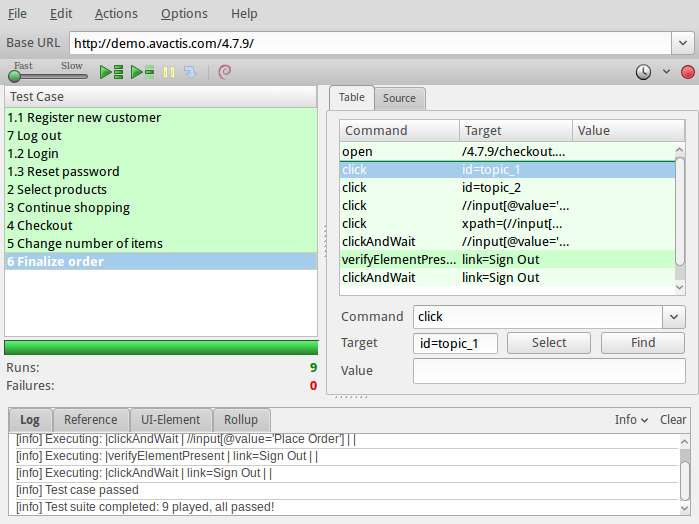
\includegraphics[scale=0.7]{TestSuitePassed}

\subsubsection{Unit test ordering}

In my test suite I've used the same order for the unit tests as listed in
the requirement. As both the username and password to be used for a new user
that will be registreted in the first TC1.1 unit test and then used for all
tests, it's crucial for the test suite to be run from the first test.
As the registration authenticates the user, it's required to sign out before
being able to perform the other tests requiring signing in.
As we have TC7 for this functionality, TC1.1 doesn't sign out, in
stead TC7 is run as the second test for this functionality being
covered by it's relevant test before being used in any tests following.

All tests following depends on the state following the previous test's completion,
TC1.2 \& TC1.3 depends on the previous test signing out at the end in order
for them to sign in at the beginning. After having tested changing password in
TC1.3, the password is changed back in order for it to be possible to run the
test suite again from TC1.2 or TC1.3 without having to restart all over with a new
user used for the tests.


With the authentication related tests completed, TC1.3 finishes with the
user still signed in, with TC2-6 all relying on continuing in their
order relying on this state.


More work could've been invested in making these tests to be run (more)
independently for the sake of convenience, but in order for them all to
run independently, one would also have to duplicate a lot of the steps
already covered by, while also being the primary task of other unit tests.
So for the sake of simplicity, we won't be doing this.

\newpage

\subsection{Transitioning manual to automated tests}

\subsubsection{Requirement Tracability Matrix}

\begin{table}[htbp]
	\begin{tabular}{|l|l|p{6cm}|}
\hline
Requirement ID & Requirement description & Remarks \\
\hline
\xintFor* #1 in \requirements\do {\ref{#1}&\ref*{name#1}&\ref*{remark#1}\\
                                  \hline }%
\end{tabular}
\end{table}

\subsubsection{Coverage}

With regards to testing whether the required functionality merely works, we do have full coverage.
Yet if taking into considerion the error situations detailed in the manual tests, we only have partial coverage.
There's also several error situations that should've been covered in these that were omitted due to lack of time.
My excuse is that I've been working alone.. :p


In addition there's a lot of other tests that could've been part of our test cases, ie. like testing of
various types of input values etcetc., but that woyuld really have been a bit too much for the scope of
this assignment.

\end{document}
